\documentclass{standalone}
\usepackage{tikz}

\begin{document}

\hspace*{\fill}
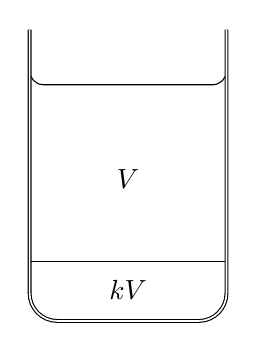
\begin{tikzpicture}
\draw[rounded corners=5] (0,3.2) --
	(0,3.0) --
	(2.5,3.0) --
	(2.5,3.2);
\draw (0,0.75) -- (2.5,0.75);
\node at (1.25,1.8) {$V$};
\node at (1.25,0.4) {$kV$};
\draw[double,rounded corners=10] (0,3.7) --
	(0,0)  --
	(2.5,0)  --
	(2.5,3.7);
\end{tikzpicture}
\hspace*{\fill}
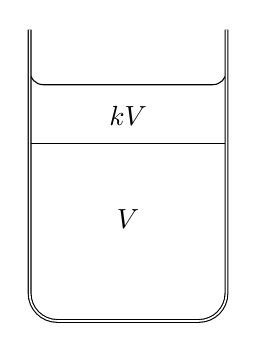
\begin{tikzpicture}
\draw[rounded corners=5] (0,3.2) --
	(0,3.0) --
	(2.5,3.0) --
	(2.5,3.2);
\draw (0,2.25) -- (2.5,2.25);	
\node at (1.25,2.6) {$kV$};
\node at (1.25,1.3) {$V$};
\draw[double,rounded corners=10] (0,3.7) --
	(0,0)  --
	(2.5,0)  --
	(2.5,3.7);
\end{tikzpicture}
\hspace*{\fill}

\end{document}